\chapter{Introduction}
\label{ch_intro}

% Define fillme
\newcommand{\fillme}{\textcolor{red}{FILL ME}}

Machine Learning (ML) is a major driver of economic value today.  Estimates suggest that ML could potentially contribute up to \$4.4 trillion annually \cite{mckinseygenai} to the global economy in the coming years, impacting sectors ranging from healthcare to finance. This large value is rooted in ML's ability to extract insights from large amounts of data and automate decision-making processes, revolutionizing traditional practices and enabling novel applications.

% ML needs data and compute
Machine learning workloads are characterized by their intensive resource requirements. They require multiple iterations over large datasets to generate progressively accurate models, a process which demands significant computational power. 
%As illustrated in Figure \ref{fig:compute_demand}, 
As a result, the compute demand of ML models has escalated over time. \romil{Add plot of ML compute demand over time} For instance, training GPT-4\cite{openai2023gpt4} in 2023 is estimated to have required 21 billion petaFLOPs\cite{mlmodelflops} of compute, representing an increase of more than $10^{7}\times$ over AlexNet, the largest model in 2012. This trend is indicative of the rising computational needs for ML, placing increasing pressure on existing resources.

% \begin{figure}
%     \centering
%     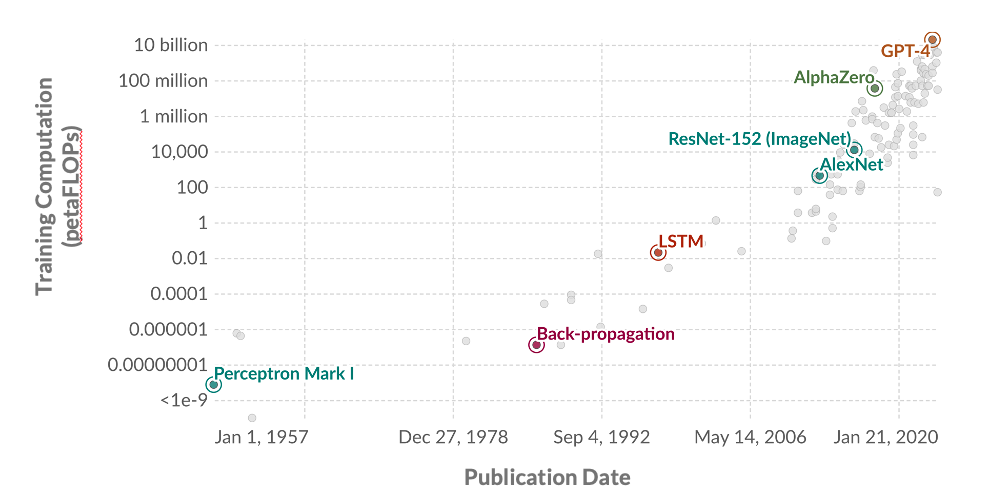
\includegraphics[width=0.7\textwidth]{intro/figures/MLCompute.png}
%     \caption{The compute demand of ML models over time. TODO - Make nicer \fillme{}}
%     \label{fig:compute_demand}
% \end{figure}

% ML has large demand
On the other hand, the supply of compute is struggling to keep up with the demand. Moore's law, which postulates that the number of transistors on a chip doubles every two years, is hitting a wall. As transistors become smaller, reaching the size of a few nanometers, physical limitations such as quantum effects and heat dissipation become significant challenges \cite{mooreslawend}. This makes it increasingly difficult to continue shrinking components at the pace predicted by Moore's Law. Worse yet, Dennard scaling, which refers to the shrinking of transistors while maintaining constant power density, has ended because of increased leakage currents and heat dissipation issues at smaller transistor sizes \cite{dennardscalingend}. Combined, these factors have led to a plateau in the growth of compute performance \cite{cpudb}.

The growing compute needs of ML and the plateauing supply of compute for training and deploying these models has created a supply-demand gap. This gap manifests in two forms - lack of resource availability and high costs of training ML models. The lack of availability \cite{gpuavailabilitywsj,gpuavailabilitytheinformation,gpuavailabilitywired} has resulted in organizations hoarding compute resources. As a corollary, the cost of training ML models has seen explosive growth, with GPT-4 costing over \$100 million to train in 2023 \cite{gpt4traincost}, compared to AlexNet which costs \$8.86 (inflation adjusted) to train in 2023\cite{mlmodelcost}. As a result, this supply-demand gap hurts the democratization of ML and hinders innovation.

% Bridging the gap by making ML more efficient - why we do so.
In this thesis, we bridge the compute supply-demand gap by developing techniques to make machine learning more resource efficient. By optimizing resource utilization, we aim to reduce the overall demand for computational power, thereby easing the pressure on the strained resource supply. By doing more with less, we can reduce the demand for compute resources. 

% Looking at the ML stack
How do we improve resource efficiency for ML? Examining the ML stack reveals opportunities across its three layers (Figure \ref{fig:ml_stack}):

\begin{figure}
    \centering
    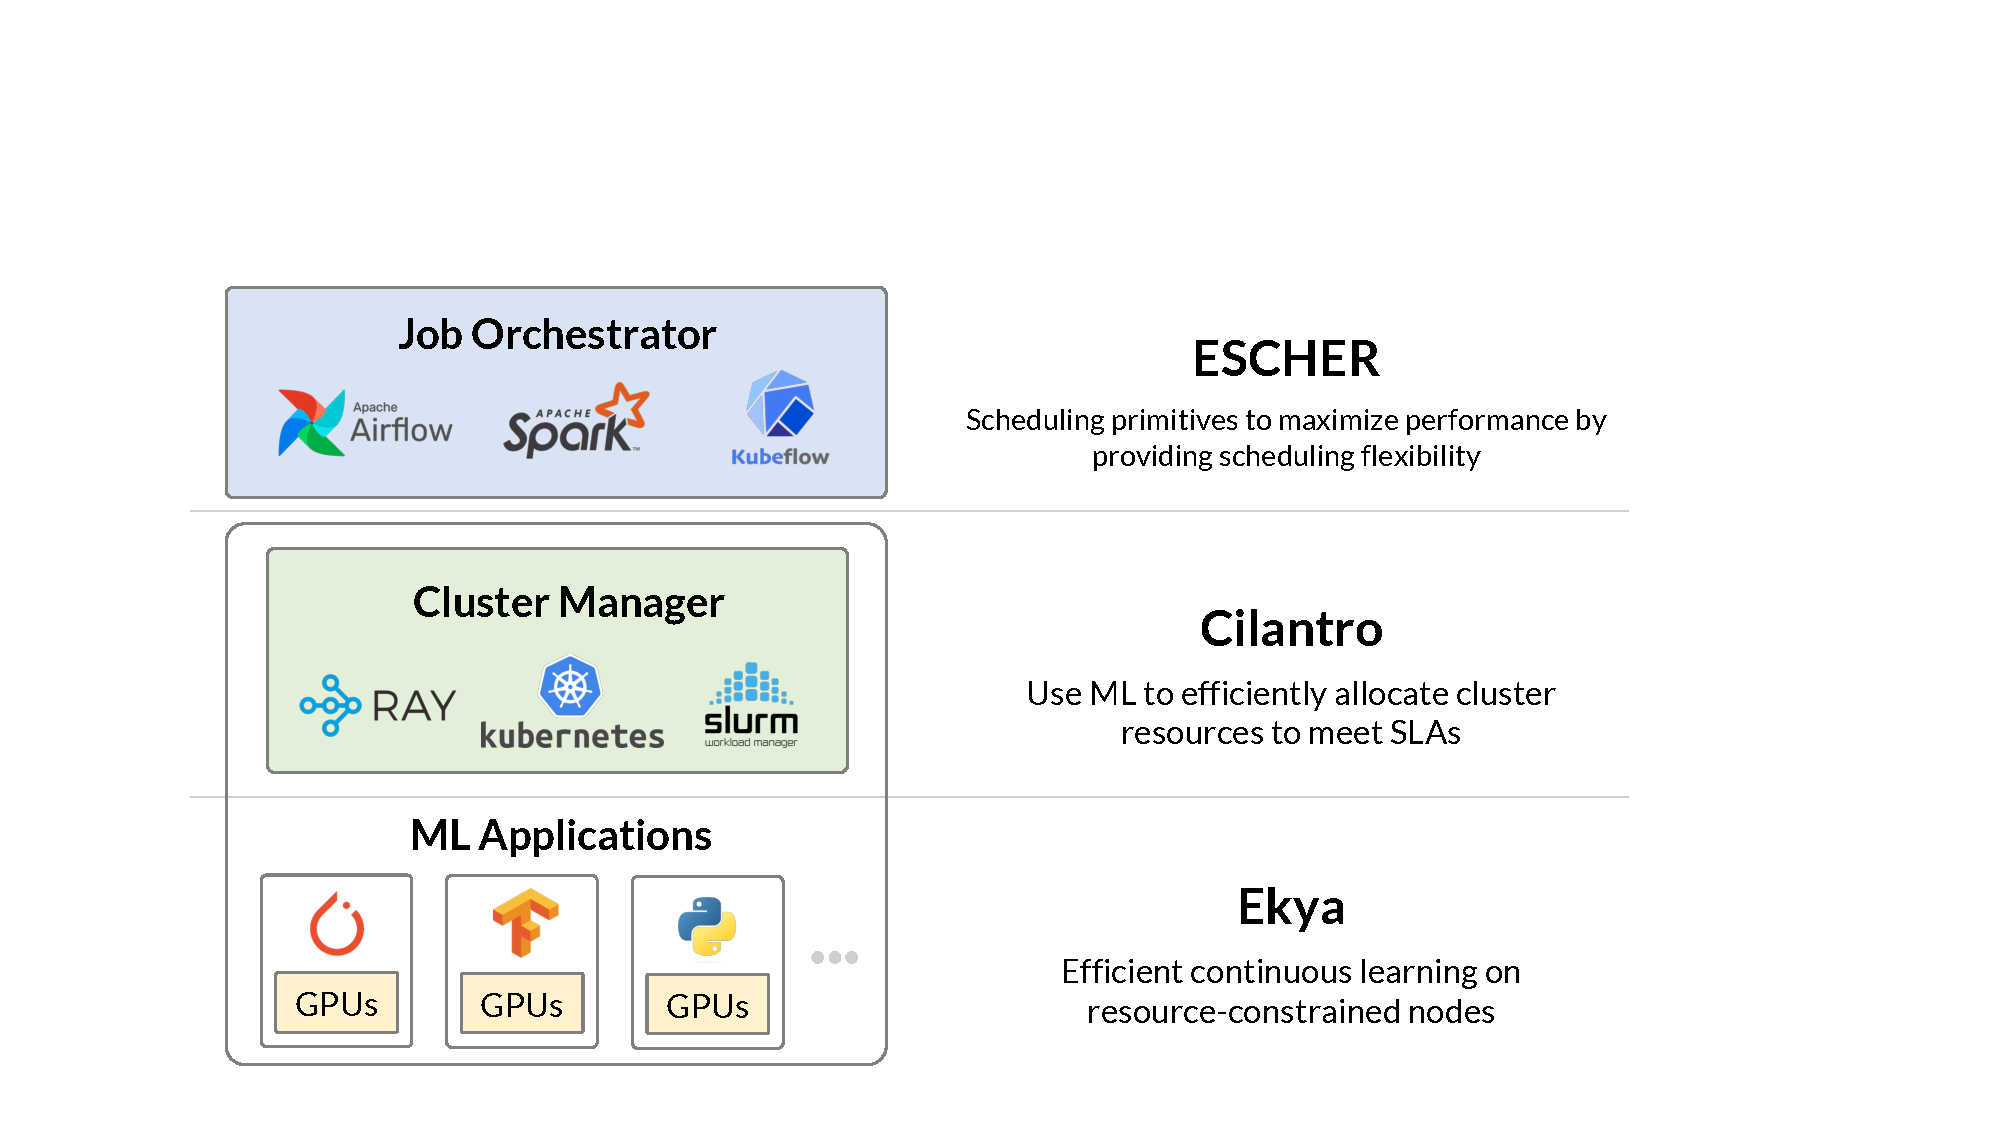
\includegraphics[width=0.9\textwidth]{intro/figures/MLStack.pdf}
    \caption{The machine learning stack spanning across the orchestration, cluster management, and ML application layers. This thesis introduces techniques and systems (listed on the right) to improve resource efficiency across all three layers.}
    \label{fig:ml_stack}
\end{figure}


\begin{enumerate}
    \item \textbf{Orchestration Layer:} This layer consists ML orchestration tooling and applications to coordinate the execution high-level business logic and low-level complex distributed training and inference tasks. Examples of such tools include Airflow\cite{airflow}, Kubeflow\cite{kubeflow} and Pytorch Distributed \cite{pytorch}. The resource efficiency of this layer is heavily dependent on its ability to leverage application-level hints for performance optimization. 
    
    \item \textbf{Cluster Management Layer:} This layer is responsible for managing and allocating resources in a cluster to run tasks submitted by the orchestration layer. It oversees scheduling jobs, book-keeping of physical resources and handling failures, if any. Examples of cluster managers include Kubernetes\cite{kubernetes}, Mesos\cite{mesos} and YARN\cite{yarn}. This layer is inherently multi-tenant, where resources must be shared among different users belonging to the same organization. As a result, maximizing resource efficiency at this layer requires careful allocation of resources across jobs belonging to different to maximize overall cluster utility.   
    
    \item \textbf{ML Application Layer:} This layer comprises ML models and their training algorithms running on specialized accelerators such as GPUs. Tools like PyTorch\cite{pytorch}, TensorFlow\cite{tensorflow} and JAX\cite{jax2018github} are commonly used for model definition and job specification. Improving resource efficiency at this layer requires optimizing the underlying ML models and the scheduling algorithms used to allocate resources to them.
\end{enumerate}

This thesis builds techniques to improve ML efficiency by rethinking how our resource allocation systems work. These techniques span all three layers of the machine learning stack.

% Ekya
At the ML application layer, we build \textbf{Ekya} (Chapter \ref{ch_ekya}) to make continuous learning, a compute-intensive but necessary technique to run high-accuracy inference, 4x more efficient. These eficiency improvements are enabled by the Thief Scheduling algorithm in Ekya, which inverts the work-stealing idea \cite{workstealing} to allow individual jobs to "steal" resources from one another. In doing so, the scheduler reallocates resources from less critical inference jobs to more impactful retraining jobs, prioritizing configurations that maximize accuracy improvements relative to resource costs. Complementing this, the Microprofiler in Ekya accurately assesses the resource demands and potential accuracy gains of various retraining configurations. This profiling enables the Thief Scheduler to make informed and efficient decisions about resource distribution. Together, the Thief Scheduler and the Microprofiler allow Ekya to effectively manage resource constraints and address data drift in edge environments, achieving the same accuracy while using 4x fewer resources.

% Cilantro - Cluster manager
At the cluster manager layer, we find that the current resource allocation model used today is inefficient. Most cluster managers are unaware of a job's performance for a given resource allocation, and instead expect users to state their resource requests when submitting jobs. However, because these requests are often best-effort estimates made by humans, they are inaccurate and lead to inefficient resource allocation. To address this, we build \textbf{Cilantro} (Chapter \ref{ch_cilantro}), which uses an online learning mechanism to form feedback loops with jobs, thereby estimating resource-to-performance mappings and adapting to load shifts. This approach alleviates the need for job profiling and allows for a variety of user- defined scheduling objectives. Cilantro's policies are uncertainty-aware, adapting to the learned models' confidence bounds. It demonstrates effectiveness in two scenarios: a multi-tenant 1000 CPU cluster, where it outperforms baselines and improves user utilities up to $1.2-3.7\times$, and a microservices setting, where it reduces end-to-end P99 latency by $0.57\times$ compared to baselines. In doing so, Cilantro marks a significant departure from traditional performance-oblivious policies, offering a more flexible, accurate, and efficient method of resource allocation.

% Escher - Orchestration layer
Finally at the orchestration layer, we discover that modern machine learning applications have very diverse scheduling requirements and their performance is highly sensitive to the underlying cluster manager's scheduling decisions.  As these applications evolve, they require \textit{scheduling flexibility} which allows them to exercise control over how their tasks are placed and executed. However, in today's systems, this \textit{scheduling flexibility} comes at the cost of simplicity. Expressing a custom scheduling need requires an application to modify the underlying monolithic scheduler in the cluster manager, a task which is inherently complex and challenging to maintain. In this thesis, we introduce \textbf{ESCHER} (Chapter \ref{ch_escher}), a cluster scheduler design that allows machine learning applications to express their scheduling requirements without the complexity of reimplementing a cluster scheduler. ESCHER introduces ephemeral resources, an abstraction which allows applications to express scheduling constraints as resource requirements. These requirements are then matched to available resources through a simple mechanism. Implemented on Kubernetes and Ray, ESCHER demonstrates the ability to express common policies found in monolithic schedulers, while also providing the flexibility for applications to easily create custom policies that were previously unsupported. % Add more results

% Future work and conclusion
In Chapter \ref{ch_conclusion}, we conclude by discussing future directions for research in this space. Specifically, we discuss the lessons learnt and explore alternative approaches to closing the compute supply-demand gap. Combined, this thesis presents a approach to addressing the compute supply-demand gap in ML through intelligent application-aware scheduling. By innovating across the ML stack, it drives efficiency in resource utilization, paving the way for sustainable and cost-effective ML in the face of its ever-growing computational demands.


% Commented out stuff

% Ekya - Specialized accelerators
% In the ML application layer, we introduce \textit{Ekya} (Chapter \fillme{}), a system for continuous learning in resource constrained environemnts. Models specialized for low resource utilization are prone to data-drift, which necessitates continuous retraining of models to maintain a high accuracy. However, this requires careful scheduling of GPU resources, since allocating inference resources to training reduces the real-time accuracy of the models. Enabled by the Thief Scheduling algorithm, Ekya intelligently allocates resources between training and inference jobs, focusing on configurations that maximize accuracy improvements for resource costs. The Microprofiler complements this by estimating resource demands and potential accuracy gains, allowing for informed and efficient scheduling decisions. This approach effectively manages resources in constrained environments, enhancing the efficiency of continuous learning for high-accuracy inference by $4\times$.

% Cilantro - Cluster manager
% At the cluster manager layer, \textbf{Cilantro} (Chapter \fillme{}) rethinks the resource allocation model for modern cluster schedulers. Instead of allocating resources based on inaccurate human-estimated demands, Cilantro uses online learning to learn the resources required by a job over time. It forms feedback loops with jobs, creating dynamic resource-to-performance mappings to estimate the resources required to achieve the job's service level objective (SLO). In doing so, Cilantro accounts for uncertainty in online models and builds a resource allocation policy that maximizes a global objective stated by the user. As a result, Cilantro marks a significant departure from traditional performance-oblivious policies, offering a more flexible and upto 3.7x more efficient method of resource allocation.

% Escher - Application layer
% Lastly, at the orchestration layer, \textbf{ESCHER} (Chapter \fillme{}) addresses the need for scheduling flexibility without complicating the underlying cluster manager. It introduces ephemeral resources, allowing applications to specify custom scheduling constraints easily. Implemented in Kubernetes and Ray, ESCHER demonstrates enhanced policy expression capabilities, balancing ease-of-use with customizability.

